\section{Implementierung}
we propose to apply just in time retrieval mechanisms to bring the content to the user in a web-based scenario.
 	first prototype is a chrome extension which proposes Europeana content based on the current user context, i.e., the current web site

 	to enrich the users browsing experience with cultural content, addiational functionality needs to be added to existing web pages, wich is called javascript-injection. by exectuing injected java-script, the look and feel of web pages can be altered and aditional information and functionality can be added.
 	altough the initial burden to install a browser extension is aliitle higher compared to the other approaches we chose to implement a browser extension because of the following advantages: the widget is limited to the wweb pages implementing it and the bookmarklet needs to be triggered on every page on which additional information is desirable, whereas the browser extension is applicable to all web pages without additional effort. Also, both, bookmarklet and widget are limited to the context of the current page and cannot account for addional inforamion source( eg browsing history), to tailor the injected cultural contents towards the users interests.

 	we decided to start with an extension for google chrome for the following reasons: according to StatCounter Google Chrome has the highest and still growing market share of 40\%. Moreover FIrefox, Safari and Opera share similar extension architectures with chrome, all based on standart web technologies, such as html, javascript and css. thus the results from a google chrome extension can easily be transfered to the afore mentioned other browsers. developing an extension for google chrome and porting the result to the browsers with a similar extension architecture will cover around 70\% of the browsers in use.

 	siehe paper über EEXCESS
 \subsection{Verwendung von AngularJS für alle Komponenten des Plugins}
 \begin{figure}
 	\centering
 	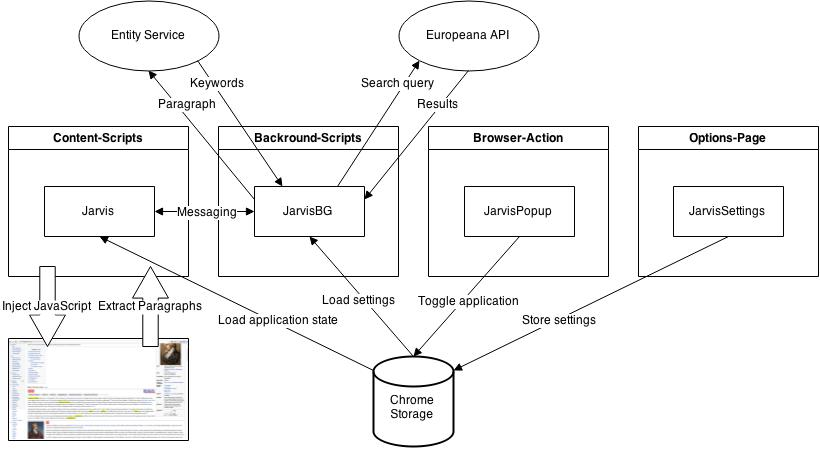
\includegraphics[width=0.8\textwidth]{Bilder/architektur.png}
 	\caption{Kommunikation der Komponenten untereinander}
 	\label{fig:architektur}
 \end{figure}
 \subsection{Bau der GUIs}
		- > Darf den Benutzer nicht zu sehr ablenken
		- > Ergebnisse müssen in der Nähe ihrer „Quelle“ angezeigt werden (proximity compatibility pricinple)
		- > Benutzer muss klar zwischen Webseite und Augmentation unterscheiden können
		- > buntes, auffälliges Design
		- > Ramping interface: Mehr Benutzerinteraktionen führen zu mehr angezeigten Informationen (Erklärung der Stages) 
 \subsection{Einbindung der REST-Services}